\documentclass{hehe}
\usepackage[table]{xcolor}
\usepackage[utf8]{inputenc}
\usepackage{longtable}
\usepackage{multirow}
\usepackage{blindtext,alltt}
\usepackage{tikz}
\usepackage{pgfplots}
\pgfplotsset{compat=1.17}
\usepackage{amssymb}
\usepackage{amsmath}
\usepackage{mathtools}
\usepackage{indentfirst}
\usepackage{footnote}
\makesavenoteenv{tabular}
\makesavenoteenv{table}
\usepackage{multirow}
\usepackage{makecell}
\usepackage[stype=amc,natbib=true,backend=bibtex,maxbibnames=20]{biblatex}

\bibliography{refs.bib}

\usetikzlibrary{arrows,decorations.markings}

\tikzstyle{basic} = [rectangle, minimum width=3cm, minimum height=0.75cm, text width=2.8cm, text centered, draw=black, fill=white]
\tikzstyle{ios} = [rectangle, minimum width=3cm, minimum height=0.75cm, text width=2.8cm, text centered, draw=black, fill=green!30]
\tikzstyle{ioe} = [rectangle, minimum width=3cm, minimum height=0.75cm, text width=2.8cm, text centered, draw=black, fill=red!30]

\makeatletter
\DeclareRobustCommand\bigop[2][1]{%
  \mathop{\vphantom{\sum}\mathpalette\bigop@{{#1}{#2}}}\slimits@
}
\newcommand{\bigop@}[2]{\bigop@@#1#2}
\newcommand{\bigop@@}[3]{%
  \vcenter{%
    \sbox\z@{$#1\sum$}%
    \hbox{\resizebox{\ifx#1\displaystyle#2\fi\dimexpr\ht\z@+\dp\z@}{!}{$\m@th#3$}}%
  }%
}
\makeatother


\newcommand{\XORsum}{\DOTSB\bigop[0.92]{\Xi}}

%% Full title
\title{Single File Compression Through Successive Bit Shifted XOR Functions}

%% Shorter title, for use in page header
\runningtitle{SBX File Compression}
\author{Rosie Bartlett}

%% The .bib file containing reference entires, for use with biblatex. CUP-INO loads the biblatex-chicago package with customisations for INO.
\addbibresource{refs.bib}

\begin{document}

\maketitle

\begin{abstract}
Compression is undoubtedly an exceptionally important part of data storage. Throughout this paper I will be exploring a new compression method that utilises XOR functions and bit shifting to compress data. This method also gives rise to compound compression, resulting in incresed efficiency.\\
\keyWords{Compression; Compund compression.}
\end{abstract}

\section{Preface}

To preface this paper, I would like to first explain the notation used throughout this paper. The method being discussed throught this paper is refered to as SBX, for successive bit shifted XOR compression. SBX uses bit shifting to compress correction keys into pairs of shorter keys and bit shift lists, or BSLs which are simply lists of integers. Since there are multiple BSLs, the BSL related to slice $n$ will be refered to as $s_n$, where the $i$\textsuperscript{th} value, starting from 1, is refered to as $s_{n,i}$. the same naming method also applies to keys, with $k_n$ being the key associated with slice $n$. One of the measures used is in relation to the length of all of the BSLs for a given file. In this instance, $s$ refers to all BSLs for the given file.

The term \textit{slice} is used extensively throughout the paper. A \textit{slice} refers to a section of the file being compressed. This is not equivalent to a \textit{file}. A \textit{file} is comprised of \textit{slices}. The term \textit{pair} is used extensively throughout and refers to a BSL calculation class and key class, and not the actual values contained within the classes. For mathematical notation, see \cref{tab:notationTable}.

\begin{table}[ht]
    \centering
    \begin{tabular}{c >{\raggedleft\arraybackslash}p{5.5cm} >{\raggedleft\arraybackslash}p{3cm}}
        \hline
        Symbol & Description & Type \\
        \Xhline{3\arrayrulewidth}
        $s_n$ & Bit shift list for file $n$ & List of integers \\
        $k_n$ & The associated key for file $n$ & Bit string \\
        $D(k_n,s_n)$ & Decoding function. See \cref{eqn:dn} & Function \\
        $\XORsum$ & Bitwise XOR shorthand. See \cref{eqn:xorSumExplain} & Operation \\
        $<<$ & Bit shift left & Operation \\
        $I_n$ & Correction key. See \cref{eqn:in} & Bit string \\
        $F_n$ & File $n$, where n$\neq0$ & Bit string \\
        $F_{0C}$ & Calculated $F_0$ for a given key and BSL pairing. This may be an incorrect $F_0$ & Bit
        string \\
        $F_0$ & Compressed file & Bit string \\
        $L(s)$ & Number of items in all bit shift strings & Integer\\
        \hline
    \end{tabular}
    \caption{Notation used throughout this paper, in order of occurrence}
    \label{tab:notationTable}
\end{table}

\section{Compression}

\begin{figure}[h!]
  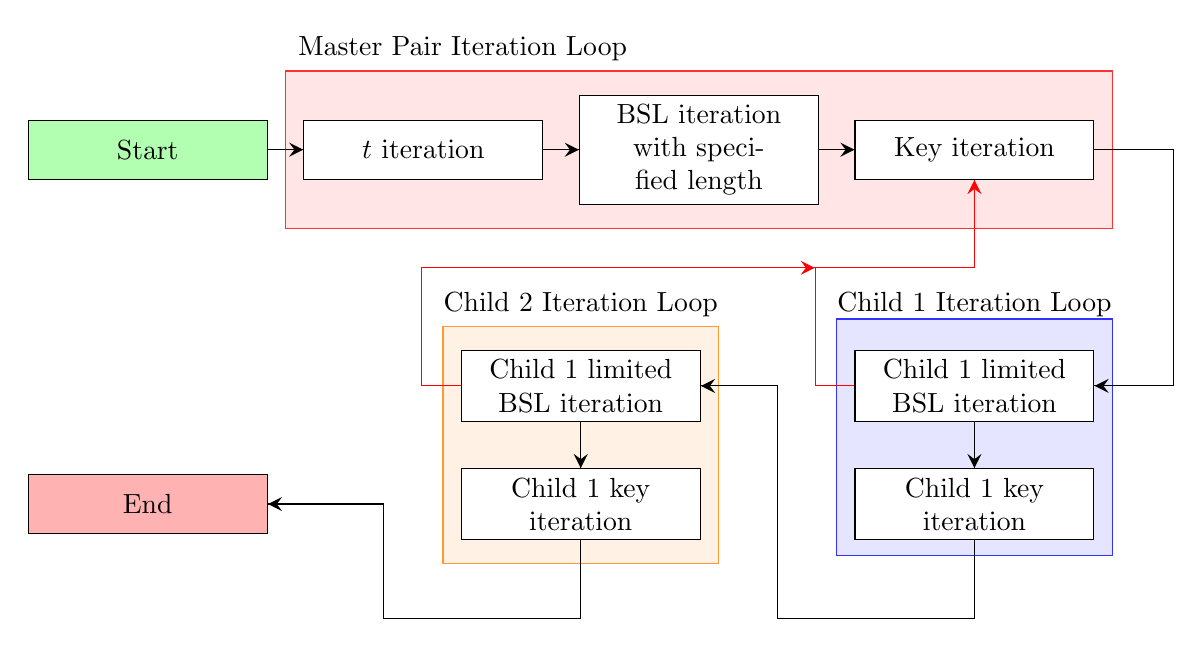
\begin{tikzpicture}[node distance=1.5cm]
    \tikzset{myptr/.style={decoration={markings,mark=at position 1 with %
    {\arrow[scale=1.6,>=stealth]{>}}},postaction={decorate}}}
    \node[above] at (0.5,1){Master Pair Iteration Loop};
    \fill[draw=red!80, fill=red!10] (-1.75,-1) rectangle  +(10.5,2);
    \node (length_iter) [basic] {$t$ iteration};
    \node (Start) [ios, left of=length_iter, xshift=-2cm] {Start};
    \node (bsl_iter) [basic, right of=length_iter, xshift=2cm] {BSL iteration with specified length};
    \node (key_iter) [basic, right of=bsl_iter, xshift=2cm] {Key iteration};

    \node[above] at (7,-2.25){Child 1 Iteration Loop};
    \fill[draw=blue!80, fill=blue!10] (5.25,-2.15) rectangle  +(3.5,-3);
    \node (child1_bsl_iter) [basic, below of=key_iter, yshift=-1.5cm] {Child 1 limited BSL iteration};
    \node (child1_key_iter) [basic, below of=child1_bsl_iter] {Child 1 key iteration};

    \node[above] at (2,-2.25){Child 2 Iteration Loop};
    \fill[draw=orange!80, fill=orange!10] (0.25,-2.25) rectangle  +(3.5,-3);
    \node (child2_bsl_iter) [basic, left of=child1_bsl_iter, xshift=-3.5cm] {Child 1 limited BSL iteration};
    \node (child2_key_iter) [basic, below of=child2_bsl_iter] {Child 1 key iteration};

    \node (End) [ioe, left of=child2_key_iter, xshift=-4cm] {End};

    \draw[myptr] (Start.east) -- (length_iter.west);
    \draw[myptr] (length_iter.east) -- (bsl_iter.west);
    \draw[myptr] (bsl_iter.east) -- (key_iter.west);

    \draw[myptr] (key_iter.east) -| ++(1cm,0) |- (child1_bsl_iter.east);
    \draw[myptr] (child1_bsl_iter.south) -- (child1_key_iter.north);
    \draw[myptr, color=red] (child1_bsl_iter.west) -| ++(-0.5cm,0) |- ++(0,1.5cm) node[anchor=west] (point) {} -| (key_iter.south);
    \draw[myptr] (child1_key_iter.south) |- ++(0,-1cm) -| ++(-2.5cm,0) |- (child2_bsl_iter.east);

    \draw[myptr] (child2_bsl_iter.south) -- (child2_key_iter.north);
    \draw[myptr, color=red] (child2_bsl_iter.west) -| ++(-0.5cm,0) |- ++(0,1.5cm) -- (point);
    \draw[myptr] (child2_key_iter.south) |- ++(0,-1cm) -| ++(-2.5cm,0) |- (End.east);
  \end{tikzpicture}
  \caption{File compression method for three files excluding preprocessing}
  \label{fig:comp_flowchart}
\end{figure}

SBX uses a parallel iterative process to compress single files. This process (see \cref{fig:comp_flowchart}) is only run once per file and returns the optimal BSLs, keys, and $F_{0c}$ for the respective file. This process is split into two parts, preprocessing and file compression. The file compression method is outlined in \cref{fig:comp_flowchart}. Please note however, that each node is representative of an iterative loop, that when ended returns to the previous node. For the child BSL iteration nodes however, once these have ended, they return to the master pair key iteration node.

\subsection{Proprocessing}

Before the file can be considered, a small amount of preprocessing must be performed. This preprocessing consists of populating two empty lists, which will be referred to as $s_0$ and $t$, as well as initialising classes. The first list to be populated, $s_0$, is an exhaustive two dimensional list of all the possible BSL values. When this list is being populated, each item added is an exhaustive list of all possible BSL values of a specific length, with this length starting at one and ending with a length of $l$. The second list, $t$, is all the different combinations of the lengths of the different BSL values for all the slices. This is ordered in ascending order by considered the sum of each list value within $t$.

For example, when $n$ is 2 and $l$ is 3, $s_0$ would be:\\\texttt{[[[0], [1], [2]], [[0, 1], [0, 2], [1, 2]], [[0, 1, 2]]]};\\and $t$ would be:\\\texttt{[[1, 1], [2, 1], [1, 2], [3, 1], [2, 2], [1, 3], [3, 2], [2, 3], [3, 3]]}.

Once this has been completed, the file can now be considered. This consists of the file being converted into slices\footnote{Each slice is the same length, and padding is added if required to allow this}, and then each slice being allocated to classes that all hold their respective slice. The first class is different to the others, as it is a master pair class instance which controls all of the compression. Each class contains more data needed for the compression such as the key length, and references to the master pair node class instance for the child nodes, and a list of references to the child nodes for the master pair node.

\subsection{File Compression}

Once the preprocessing has finished, then the compression can begin. The compression is controlled by the master pair node, and begins begins by iterating over each of the items in t. For each of these, it iterates over each of the possible BSL values with a length specified by the first item in the current iteration of t. For each of these iterations, every possible value for the key is iterated over and $F_{0c}$ is calculated, see \cref{eqn:f0c}, using the current value of the BSL and the current value of the key.

\begin{equation}\label{eqn:f0c}
  F_{0c}=F_1 \oplus D(k_1\oplus s_1)
\end{equation}
\begin{equation}\label{eqn:in}
  I_n=F_n\oplus F_{0c}
\end{equation}

Once $F_{0c}$ has been calculated, the master pair begins iterating over each of the child nodes. For each child node iteration, a small amount of preprocessing must be performed first to enable checks later on. This preprocessing contains calculating $I_n$, and then the offset of the first and last non-zero bit in $I_n$. Once these have been calculated, the child begins iterating over all possible BSL values with a length specified in the current iteration of $t$ in the master class. The index of the child within the master pair class' list of children is the index used in retrieving the current BSL length to iterate over, with the first child accessing the second item in the current iteration of $t$, the first value having already been used by the master pair class.

\begin{equation}\label{eqn:dn}
  D(k_n,s_n)=\XORsum_{i=1}(k_n << s_{n,i})
\end{equation}
\begin{equation}\label{eqn:xorSumExplain}
  \XORsum_{i=1}^m(x_i)=x_1\oplus x_2\oplus \dots \oplus x_m
\end{equation}

It is here that the first efficiency check is performed. The first value in the current BSL value has to be less than or equal to the index of the first non-zero bit in $I_n$, and the last value in the current BSL added to the length of the key must be larger than or equal to the index of the last non-zero bit in $I_n$. This check ensures the the current BSL is able to produce a non-zero bit in the lowest and highest index required. If this check is passed, then the child node then attempts to calculate a key that, when paired with the respective BSL and then passed into \cref{eqn:dn}, would result in $I_n$.

To attempt to calculate the required key for the current BSL, the process first begins by considering the first bit in $I_n$. This bit is then saved as the current calculated key, and the precess moves onto the next bit. From this point onwards the calculation becomes slightly more complicated. After the first bit, the process first calculates $D(k_n, s_n) \oplus I_n$, and then considers the current bit being calculated. This bit is then added to the end of the previously saved key. This is a bitwise process that relies upon the previous bits having been calculated so that there is a maximum of one unknown bit that can be calculated. This process does include checks to improve efficiency, such as only using values in the BSL that could affect the current bit being calculated.

However, this calculation method is not perfect and errors can be introduced throughout. Because of this, once the key calculation has been performed, the result of the calculation is passed into the key expansion method, $D$, along with the respective BSL, the result of which is compared against $I_n$. If these are identical then the child returns true to the master pair node, which then continues iterating over the remaining children. If none of the child BSL values could be used, then a new key is generated and the process begins from the first child. Once all children have successfully been iterated over, the master pair and all child nodes save their values and the iterative process is ended. This can be done due to the sorting of $t$ in the preprocessing. Since $t$ was sorted by the sum of each of the elements, then once all children have successfully been iterated over, then there cannot be a lower values of $L(s)$ for the current set of files, and so iteration is ended.

\subsubsection{Example of SBX Compression of a Correction Key}

Given $F_{0c}$=\texttt{10110101} and $F_n$=\texttt{11001000}, therefore the long key must be \texttt{01111101}. However, this long key can be compressed, and represented using the key \texttt{11001} and the BSL \texttt{[0, 2]}. To expand the key and BSL pair into the long, or intermediate, key, which is XOR-ed with the master file to produce the file related with this specific BSL and key pair, the BSL is used one item at a time in the following manner once the long key has been initialised to 0. First the key is bit shifted left by the current value in the BSL. This is then XOR-ed with the long key and replaces the previously stored long key value. Using the example previously given, this would result in \texttt{11001} being first bit shifted by 0 to the left resulting in \texttt{11001}. This is then XOR-ed with the initialised long key value of 0, resulting in the long key now having a value of \texttt{11001}. The next value in the BSL is 2, so the key is bit shifted left by 2 resulting in \texttt{1100100}. This is then XOR-ed with the long key resulting in \texttt{01111101}, which is the desired long key for this $F_0$ and $F_n$.


\section{Expansion}

Due to the simplicity of SBX, file expansion is an exceptionally quick process. The expansion begins by parsing the compressed file and splitting this into the relevant sections detailed in \autoref{sec:CompressedLayout}. Once this has been completed, the program now has access to $F_0$, $k$, and $s$, and can therefore expand the file. This expansion, using \cref{eqn:expand}, is fairly simple and does not require any complex and time consuming calculation, thus making expansion exceptionally fast. The speed of expansion has been quantified in \autoref{sec:results}.

\begin{equation}\label{eqn:expand}
  F_n=F_0\oplus D(k_n, s_n)
\end{equation}

\section{Compund Compression}

Since SBX can compress any size of data, it only makes sense that to improve the efficiency of the compression, the keys usd withing SBX would be compressed themself, thus giving rise to compund compression. Compund compression is only applied to the keys of a compressed file.


\section{Compressed File Data Layout}
\label{sec:CompressedLayout}

\begin{table}[ht]
    \centering
    \begin{tabular}{c c | c | >{\raggedright\arraybackslash}p{7.5cm}}
        \hline
         & Bit offset & Length & Description \\
        \Xhline{3\arrayrulewidth}
        \cellcolor{red} & 0 & 4 & Length of each file passed into the compression function, $\frac{l}{8}$, in bytes \\
        \cellcolor{blue} & 4 & 1 & Boolean representing a nested compression of the key \\
        \cellcolor{blue} & 5 & $l+1$ & Key $k_n$ \\
        \cellcolor{blue} & $6+l$ & 2 & Length of $s_n$, $L(s_n)$ \\
        \cellcolor{blue} & $8+l$ & $L(s_n)\log_2l$ & BSL $s_n$ \\
        \cellcolor{orange} & -4 & 4 & Padding to remove \\
        \hline
    \end{tabular}
    \caption{Bit offsets and their related description within an SBX file}
    \label{tab:dataLayout}
\end{table}

The data layout of SBX compressed files has been constructed to alow for a maximum efficiency in compression, but this does come at a slight cost. SBX can only compress data that is stored in bytes, and thus cannot handle data that includes a non integer value of bytes. This would seem to contradict some of the resuts in \autoref{sec:results}, however the results given are only for compression and do not include data storage.

In \cref{tab:dataLayout}, there are two sections, indicated by the two different colours. The first section, indicated with red, is a header section that contains the value of $\frac{l}{8}$ used when the file was compressed; or alternatively the number of bytes in each of the compressed files. This section is included at the start of all compressed sections, not just at the start of the compressed file. The second section, indicated in blue, is a repeatable section containing data on a single compressed file. The first bit is a boolean that, if true, indicates that the key of this compressed file has itself been compressed. The next part is the key which may itself need to be expanded. The length of the key in \cref{tab:dataLayout} is given as $l+1$, however this may not be true. The key will have a length of $l+1$ only if the key has not been compressed, otherwise the key will have a different length.

After the key is the length of the BSL related to the current section, followed by the BSL itself. This section is repeatable. After all of the compressed file sections have been parsed, this leaves the final 4 bits, which represent the padding added to the first compressed file to allow for the most efficient compression. This is removed from the first file before all the compressed files are concatenated together. The offset for the padding to remove section is a negative since this cannot be given as a general formula for all compressed files, and as such has been given relative to the end of the file.


\section{Results}
\label{sec:results}

To evaluate the effectiveness of SBX, it was run on several different sets of data, each set having a different batch and file size. The code was run on a three node raspberry pi cluster, appendix time me thinks for detailed specs, and times for each compression have been included. Each set of data contained 1000 pseudo-randomly generated files. The generated files were not individually generated, rather a single integer was generated from 0 to $nl$ inclusively, which was then sliced into $n$ seperate files.

\section{Future Work}

Whilst SBX can be efficient for large files, it is still exceptionally slow in comparison to common compression systems, such as ZIP files, which will require further development to achieve similar compression times. I am continually developing SBX to improve efficiency, and as sure that with further developemnt, SBX will become singificantly more efficient

%% Optional appendix
\appendix
\section{Pseudo Code}

This appendix is to give a general overview of the code used for SBX in the form of pseudo code. For the source code of SBX, a link is provided in the footer on the first page of the paper.


\section{Raspberry Pi Cluster Specifications}
This appendix details the specifications of the Raspberry Pi cluster that SBX was tested upon.

\begin{itemize}
  \item \textbf{Master Node}:\\
  \begin{itemize}
    \item Raspberry Pi model B
    \item Something else?
  \end{itemize}
\end{itemize}

\section*{Author}
\begin{authorbio}

\textbf{Rosie Bartlett} is a currently a student and is still developing SBX. She can be reached at abc@xyz.edu. GitHub is also a good way to keep up with the current version of SBX.
\end{authorbio}

\section*{Acknowledgements}
I would like to thank the developers of MPI for Python \cite{DALCIN20051108} which was used extensively throughout this project. I would also like to thank the peoples who helped me with writing this paper and their advice given in relation to the subject. Merci beaucoup Sophie.

\printbibliography

\end{document}
